\chapter*{Proposition 2}
\label{prop:2}

\begin{figure*}[ht]
    \begin{center}
    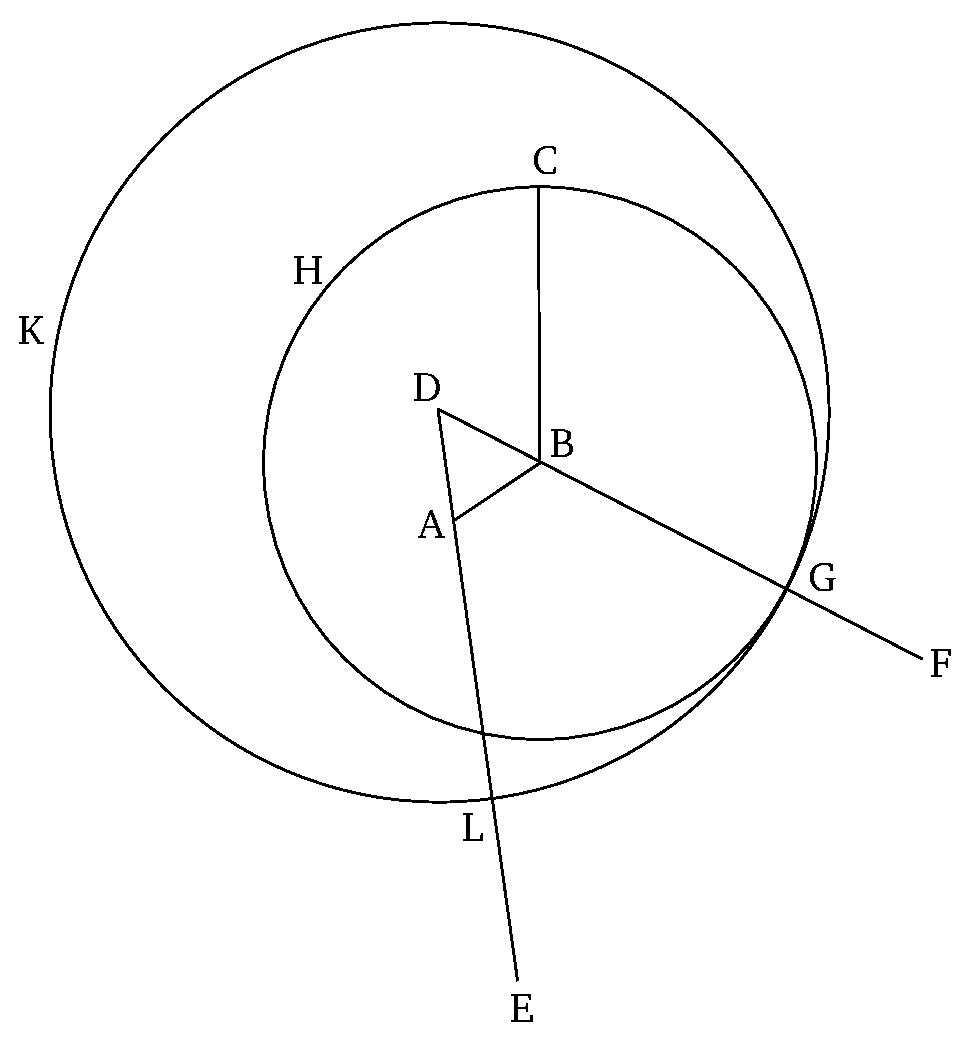
\includegraphics[width=0.5\linewidth]{figures/fig02e.eps}
    \label{fig:prop_2}
    \end{center}
\end{figure*}

To place a straight-line equal to a given straight-line at a given point (as an extremity).

Let $A$ be the given point, and $BC$ the given straight-line. So  it is required to
place a straight-line at point $A$ equal to the given straight-line $BC$.

For let the straight-line $AB$ have been joined from point $A$ to point $B$ [Post.~\ref{post:1}], and let the
equilateral triangle $DAB$ have been been constructed upon it [Prop.~1.1].  And let the
straight-lines $AE$ and $BF$ have been produced in a straight-line with $DA$ and $DB$  (respectively) [Post.~\ref{post:2}].
And let the circle $CGH$ with center $B$ and radius $BC$ have been drawn
[Post.~\ref{post:3}], and again let the circle $GKL$ with center $D$ and radius $DG$ have been drawn [Post.~\ref{post:3}].

Therefore, since the point $B$ is the center of (the circle) $CGH$, $BC$ is equal to 
$BG$ [Def.~\ref{def:5}]. Again, since the point $D$ is the center of the circle $GKL$, $DL$ is equal to $DG$ [Def.~\ref{def:5}]. And within these,  $DA$ is equal to $DB$. Thus, the remainder $AL$ is equal to the remainder $BG$ [C.N.~\ref{cn:3}]. But $BC$ was also shown (to be)  equal to $BG$. Thus,  $AL$
and $BC$ are each equal to $BG$. But things equal to the same thing are also equal to one another [C.N.~\ref{cn:1}]. Thus, $AL$ is also equal to $BC$.

Thus, the straight-line $AL$, equal to the given straight-line $BC$,
has been placed at the given point $A$. (Which is) the very thing it was required to do.

\section*{Commentary}

\begin{proposition}\label{proposition_2}\lean{Elements.Book1.proposition_2}\leanok
    $B$ and $C$ are two distinct points on a line $BC$. $A$ is a point different from $B$. There must be a point $L$, s.t. $|AL| = |BC|$.
\end{proposition}
\begin{proof}
    \uses{proposition_1}\leanok
    See the original proof by Euclid.
\end{proof}

Euclid omitted the degenerated case where $A$ is the same as $B$.

\begin{proposition}\label{proposition_2'}\lean{Elements.Book1.proposition_2'}\leanok
    $B$ and $C$ are two distinct points on a line $BC$. For any point $A$, there must be a point $L$, s.t. $|AL| = |BC|$.
\end{proposition}
\begin{proof}
    \uses{proposition_1,proposition_2}
    \leanok
    When $A = B$, we can just take $L = C$.
    When $A \neq B$, we apply Prop.~\ref{proposition_2}.
\end{proof}